%%
%% Background
%%
\section{Background}
\label{sec:background}

This section introduces the foundational concepts of quantum computation relevant to our work, provides an overview of the QuantumC compiler that we extend, and describes the quantum arithmetic implementations that we compare.

\subsection{Quantum Computing Preliminaries}
\label{sec:quantum-preliminaries}
In quantum computing, the fundamental unit of information is the \emph{qubit}, whose state is a superposition of two basis states: $|\psi\rangle = \alpha|0\rangle + \beta|1\rangle$, where $\alpha$ and $\beta$ are complex amplitudes satisfying $|\alpha|^2 + |\beta|^2 = 1$~\cite{nielsen-chuang}. Multiple qubits can be grouped into \emph{quantum registers} to represent integer values, analogous to how classical variables are stored in processor registers.

Quantum computation proceeds by applying \emph{quantum gates}, which are unitary operators that evolve the system state. In the circuit model, qubits are depicted as horizontal lines, gates as operations applied to one or more qubits, and computation flows from left to right. Common gates include single-qubit operations (X, H, phase rotations) and multi-qubit operations (CNOT, Toffoli).

Two fundamental constraints distinguish quantum from classical computation. First, quantum operations are inherently \emph{reversible}: since gates are unitary, applying the adjoint $U^\dagger$ recovers the original state. This implies that variables cannot be directly overwritten; intermediate values must be preserved or explicitly uncomputed. Second, the \emph{no-cloning theorem}~\cite{no-cloning} forbids duplicating arbitrary quantum states, eliminating the classical notion of fan-out for variable copying.

These constraints have direct implications for quantum circuit design. Since intermediate values cannot be discarded, quantum algorithms must carefully manage ancillary storage and uncomputation. The quality and cost of a quantum circuit are commonly evaluated using metrics such as \emph{qubit count} (width), \emph{circuit depth} (critical path length), and \emph{gate count}.

\subsection{Translating Imperative Programs to Quantum Circuits}
\label{sec:c-to-quantum}
Compiling a classical imperative language such as C into quantum circuits poses several fundamental challenges. The most significant is \emph{reversibility}: while classical programs freely overwrite variables, quantum operations are unitary and thus inherently reversible. A statement like \texttt{x = x + 1} cannot be directly implemented, as overwriting destroys the previous value of \texttt{x}. Similarly, the no-cloning theorem prevents duplicating quantum states, so the classical notion of copying a variable into multiple locations is not available.

These constraints are addressed by adopting Static Single Assignment (SSA) form, where each variable is assigned exactly once. Under this model, each variable in the source program is mapped to a dedicated quantum register, and each arithmetic operation becomes a quantum gate (or sequence of gates) that reads from input registers and writes to a fresh output register. The result of the computation is extracted through measurement at the end of the circuit.

\begin{figure}[h]
\centering
\begin{minipage}[c]{0.42\linewidth}
\begin{lstlisting}[language=C, basicstyle=\ttfamily\footnotesize, frame=none]
int main() {
    int a = 2;
    int b = 3;
    int prod = a * b;
    int res = prod + 1;
    return res;
}
\end{lstlisting}
\end{minipage}%
\hfill
\begin{minipage}[c]{0.56\linewidth}
\centering
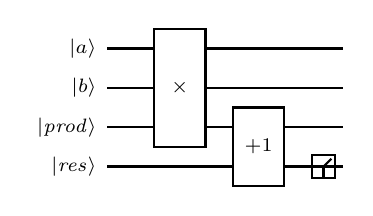
\begin{tikzpicture}[thick, scale=0.5]

% Registers
\draw (0,4) -- (6,4);
\draw (0,3) -- (6,3);
\draw (0,2) -- (6,2);
\draw (0,1) -- (6,1);

% Labels
\node[left, font=\scriptsize] at (0,4) {$|a\rangle$};
\node[left, font=\scriptsize] at (0,3) {$|b\rangle$};
\node[left, font=\scriptsize] at (0,2) {$|\mathit{prod}\rangle$};
\node[left, font=\scriptsize] at (0,1) {$|\mathit{res}\rangle$};

% Multiplication block (covers a, b, prod)
\draw[fill=white] (1.2,1.5) rectangle (2.5,4.5);
\node[font=\scriptsize] at (1.85,3) {$\times$};

% Addition block (covers prod, res)
\draw[fill=white] (3.2,0.5) rectangle (4.5,2.5);
\node[font=\scriptsize] at (3.85,1.5) {$+1$};

% Measurement symbol (meter style)
\draw (5.2,0.7) rectangle (5.8,1.3);
\draw (5.5,0.7) -- (5.5,1.0);
\draw (5.5,1.0) -- (5.7,1.2);

\end{tikzpicture}
\end{minipage}
\caption{Example of a C program and its corresponding quantum circuit. Each variable is mapped to a quantum register, while arithmetic operations are realized as quantum gates. The return value is obtained through measurement.}
\label{fig:c-to-circuit}
\end{figure}

Figure~\ref{fig:c-to-circuit} illustrates this mapping with a simple example. The C program declares two variables, computes their product, adds a constant, and returns the result. In the quantum circuit, each variable (\texttt{a}, \texttt{b}, \texttt{prod}, \texttt{res}) corresponds to a separate quantum register. The multiplication and addition operations are implemented as quantum gates that preserve the input values while writing the result to a new register. This structure directly reflects SSA semantics: no register is ever overwritten.

QuantumC~\cite{quantumc} implements this approach using an MLIR-based compilation pipeline~\cite{mlir,xdsl}. The compiler parses C source code, generates an SSA-based intermediate representation, translates arithmetic and control-flow operations into quantum gates, and exports the circuit in OpenQASM~\cite{openqasm} format. However, the current implementation supports only scalar integer operations and does not handle arrays, vectors, or matrices---the gap that our extension addresses.

\subsection{Quantum Arithmetic}
\label{sec:quantum-arithmetic}
Quantum arithmetic subroutines are essential building blocks in many quantum algorithms. In Grover's search~\cite{grover}, arithmetic comparators are used within oracles to mark target states satisfying numerical conditions. Shor's factoring algorithm~\cite{shor} relies on modular exponentiation, which decomposes into sequences of modular additions and multiplications. The HHL algorithm~\cite{hhl} for solving linear systems uses arithmetic operations to manipulate eigenvalues during matrix inversion. More broadly, any quantum algorithm that processes classical data encoded in quantum registers requires arithmetic primitives to manipulate those values.

Addition is the most basic arithmetic operation, and two main approaches exist for its quantum implementation.

\textbf{QFT-based addition.} The approach introduced by Draper~\cite{draper-qft} performs addition in the Fourier basis. The target register is first transformed via the Quantum Fourier Transform (QFT), then the addend is incorporated through controlled phase rotations, and finally the inverse QFT is applied to return to the computational basis. This method does not require ancilla qubits for carry propagation, as the carry information is encoded in the phase of the quantum state.

\textbf{Ripple-carry addition.} The approach proposed by Cuccaro et al.~\cite{cuccaro-ripple} follows the classical model of carry propagation. It uses a sequence of majority and unmajority gates, implemented with Toffoli (CCX) and CNOT gates, to propagate the carry bit through the register. This method requires ancilla qubits to store intermediate carry values but operates entirely in the computational basis without requiring the QFT.

To illustrate, adding $2 + 3$ with 3-qubit registers involves encoding the operands as $|010\rangle$ and $|011\rangle$. The addition circuit---whether QFT-based or ripple-carry---transforms these inputs and produces $|101\rangle$ (decimal 5) in the output register, while preserving the original operands for reversibility.

Other arithmetic operations in our compilation flow are built upon addition. Subtraction is performed via two's complement negation followed by addition. Multiplication can be implemented through repeated additions (shift-and-add) or using QFT-based techniques with controlled-controlled phase rotations.

The two addition approaches present different trade-offs in terms of qubit count, circuit depth, and gate composition. These trade-offs depend on the target hardware characteristics, such as native gate sets and qubit connectivity. Our extended compiler supports both backends, and we present a comparative analysis in Section~\ref{sec:results}.
